\newthought{\textbf{Nadzura Kumaira - 2020903430030 - TRKJ 3B}}

\newday{\textbf{1 Desember 2022}- Instalasi Apache Hadoop}
\begin{enumerate}
\item Kendala dan Solusi
\newline berada di perintah hadoop version dimana ketika dilakukan perintah itu tidak keluar,tapi saya membuat ulang dan akhirnya bisa

\item Kesimpulan
\newline jangan ada perintah yang ketinggalan karena itu membuat error.

\begin{figure}
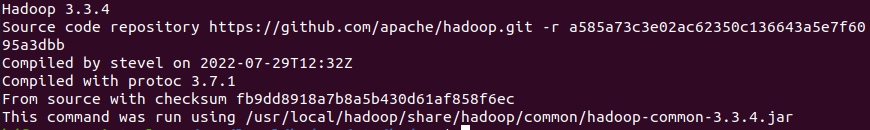
\includegraphics[width=\textwidth]
{NadzuraKumaira/hadoop version}
\caption{hasil dari hadoop version}
\label{gam:perkuliahan-25-11}
\end{figure}
\end{enumerate}

\newday{\textbf{2 desember 2022}konfigurasi apache hadoop}
\begin{enumerate}
\item Kendala dan Solusi
\newline jangan lupa sertakan <configuration> dan </configuration> setiap membuat sudo nano nama-file.
\item Kesimpulan
\newline di perhatikan tanda petik jangan ada yang terbalik.

\begin{figure}
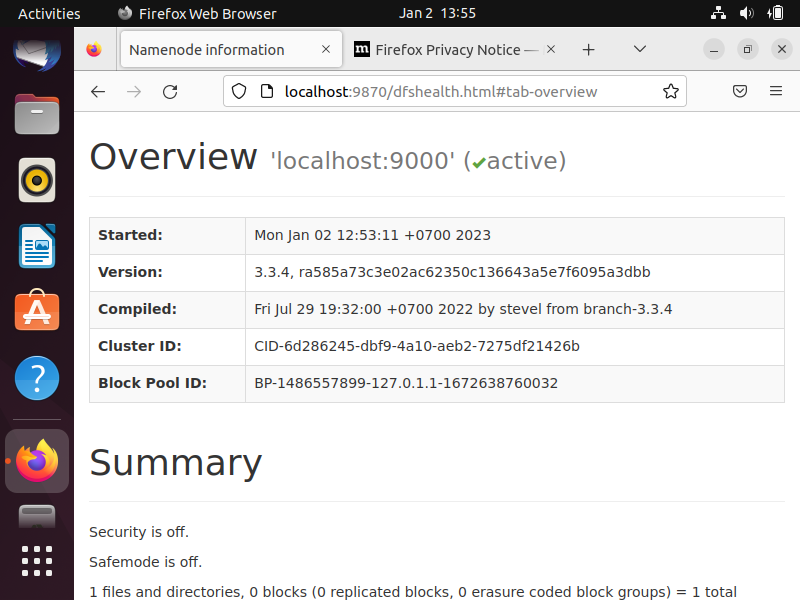
\includegraphics[width=\textwidth]
{NadzuraKumaira/localhost}
\caption{hasil dari localhost} 
\label{gam:perkuliahan-20-11}
\end{figure}

\begin{figure}
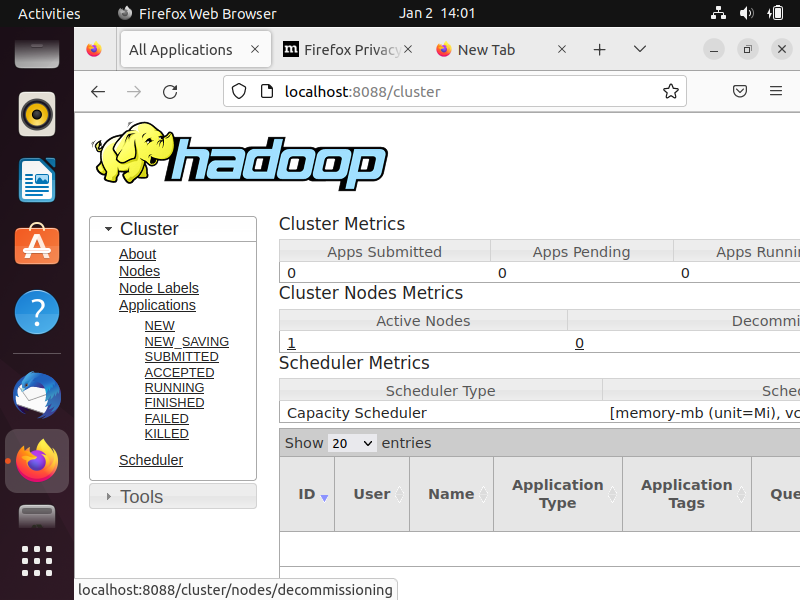
\includegraphics[width=\textwidth]
{NadzuraKumaira/localhost888}
\caption{hasil dari localhost888}
\label{gam:perkuliahan-20-11}
\end{figure}
\end{enumerate}

\newday{\textbf{8 desember 2022}}
\begin{enumerate}
\item Kendala dan Solusi
\item Kesimpulan

\begin{figure}
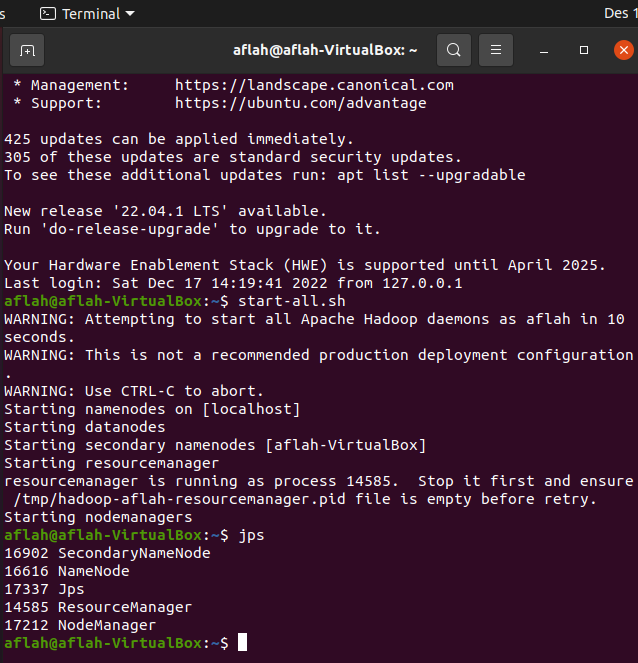
\includegraphics[width=\textwidth]
{NadzuraKumaira/jps}
\caption{chek jps}
\label{gam:perkuliahan-25-11}
\end{figure}
\end{enumerate}

\newday{\textbf{9 desember 2022}}
\begin{enumerate}
\item Kendala dan Solusi
\item Kesimpulan
\begin{figure}
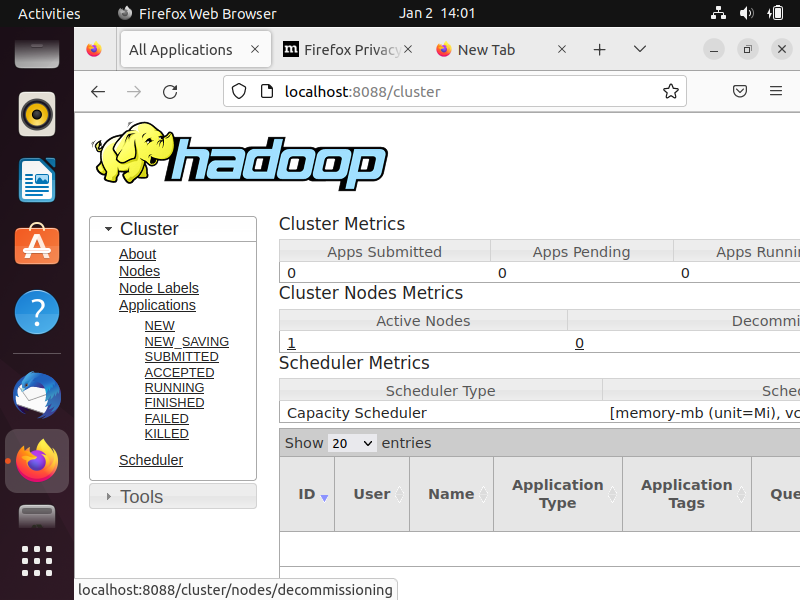
\includegraphics[width=\textwidth]
{NadzuraKumaira/localhost888}
\caption{hasil dari localhost888}
\label{gam:perkuliahan-20-11}
\end{figure}
\end{enumerate}

\newday{\textbf{15 desember 2022}program wordcount bawaan hadoop}
\begin{enumerate}
\item Kendala dan Solusi
\newline poin ke-3 jangan lupa tambah kata sudo nano.
\item Kesimpulan
\newline jangan ada perintah yang ketinggalan.

\begin{figure}
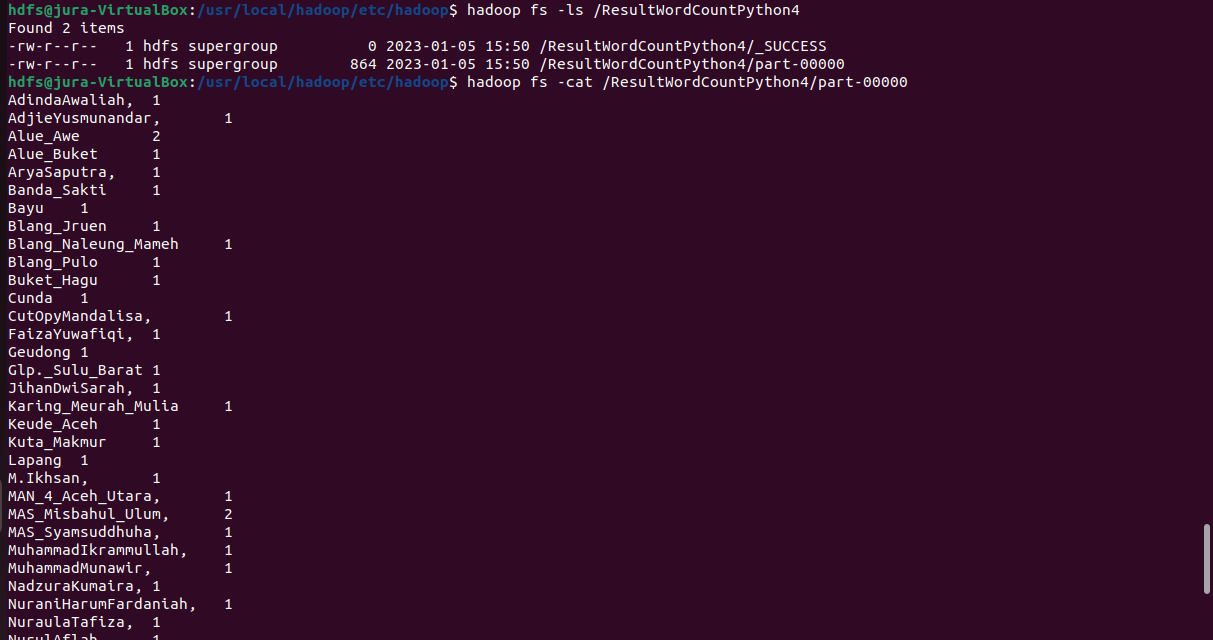
\includegraphics[width=\textwidth]
{NadzuraKumaira/hasilresultwordcount}
\caption{hasil dari hasilresultwordcount}
\label{gam:perkuliahan-10-11}
\end{figure}
\end{enumerate}

\newday{\textbf{16 desember 2022}program wordcount dengan java}
\begin{enumerate}
\item Kendala dan Solusi
\newline jangan ada perintah yang ketinggalan atau akan pusing sendiri.
\item Kesimpulan
\newline berusaha jangan mudah menyerah.

\begin{figure}
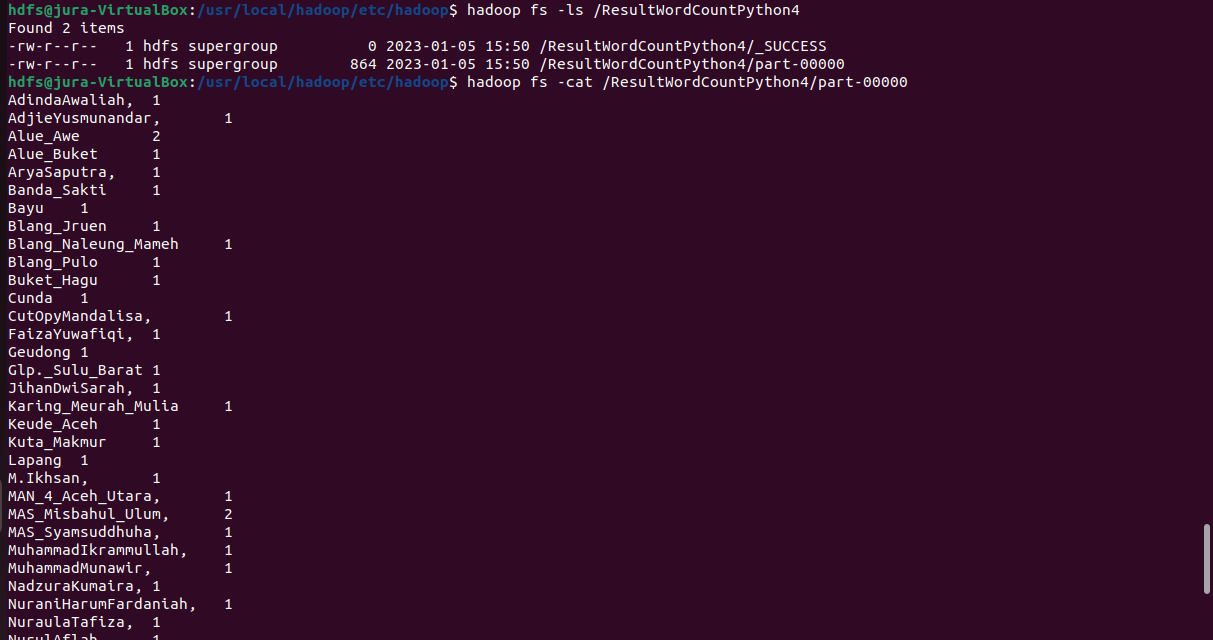
\includegraphics[width=\textwidth]
{NadzuraKumaira/hasilresultwordcount}
\caption{hasil dari hasilresultwordcount}
\label{gam:perkuliahan-17-11}
\end{figure}
\end{enumerate}

\newday{\textbf{22 desember 2022}instalasi apache spark(pyspark)}
\begin{enumerate}
\item Kendala dan Solusi
\newline jaringan wifi harus bagus agar berhasil
\item Kesimpulan
\newline jangan panik kalau macet.

\begin{figure}
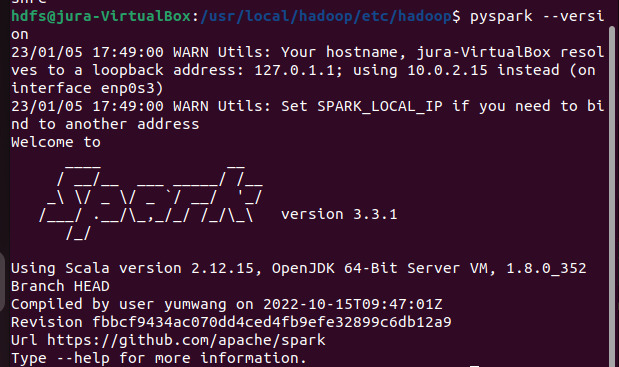
\includegraphics[width=\textwidth]
{NadzuraKumaira/pyspark}
\caption{hasil dari pyspark}
\label{gam:perkuliahan-24-11}
\end{figure}

\begin{figure}
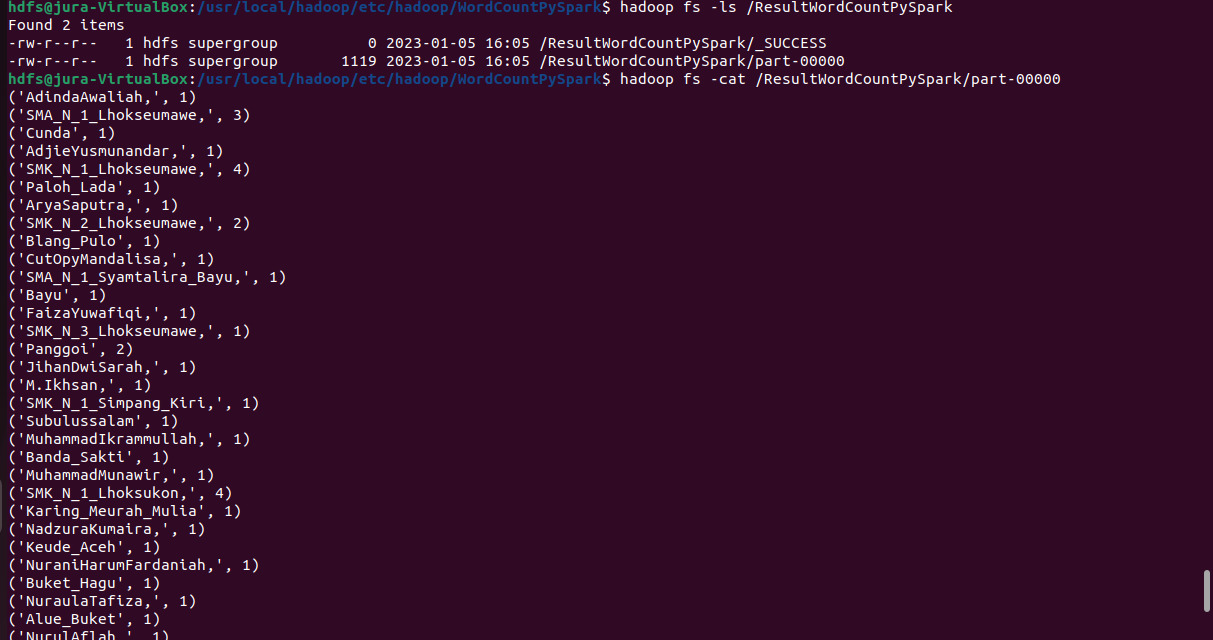
\includegraphics[width=\textwidth]
{NadzuraKumaira/hasilpyspark}
\caption{hasil dari hasilpyspark}
\label{gam:perkuliahan-24-11}
\end{figure}
\end{enumerate}

\newday{\textbf{23 desember 2022}program wordcound dengan python}
\begin{enumerate}
\item Kendala dan Solusi
\newline di perhatikan tanda petiknya.
\item Kesimpulan
\newline tanda petik bikin error.

\begin{figure}
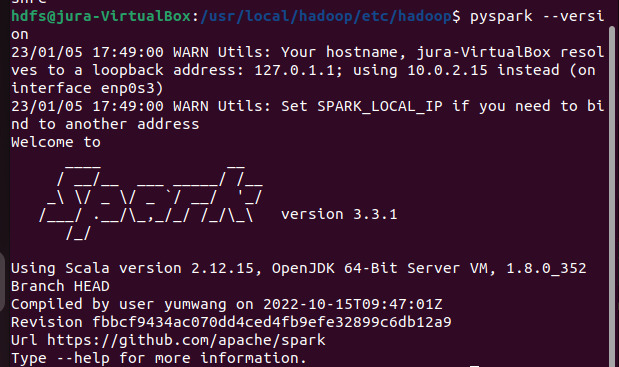
\includegraphics[width=\textwidth]
{NadzuraKumaira/pyspark}
\caption{hasil dari pyspark}
\label{gam:perkuliahan-8-12}
\end{figure}

\begin{figure}
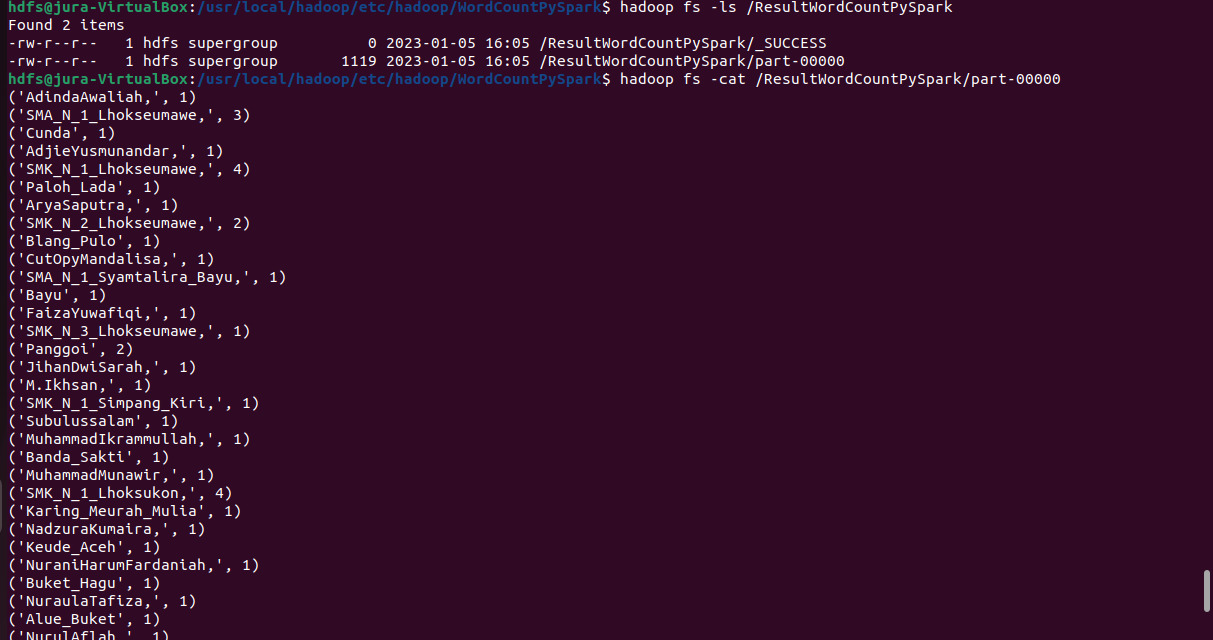
\includegraphics[width=\textwidth]
{NadzuraKumaira/hasilpyspark}
\caption{hasil dari hasilpyspark}
\label{gam:perkuliahan-8-12}
\end{figure}
\end{enumerate}

\newday{\textbf{15 desember 2022}tugas individu}
\begin{enumerate}
\item Kendala dan Solusi
\newline di perhatikan tanda petiknya.
\item Kesimpulan
\newline tanda petik bikin error.

\begin{figure}
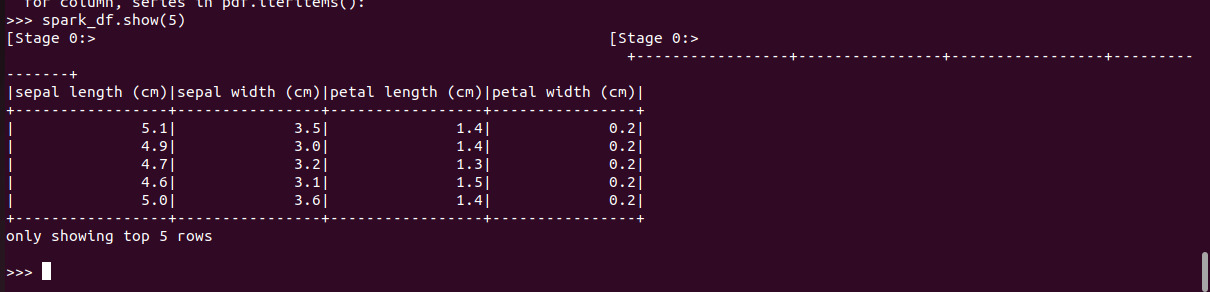
\includegraphics[width=\textwidth]
{NadzuraKumaira/tabel1}
\caption{hasil dari tabel1}
\caption{hasil dari tabel1}
\label{gam:perkuliahan-15-12}
\end{figure}

\begin{figure}
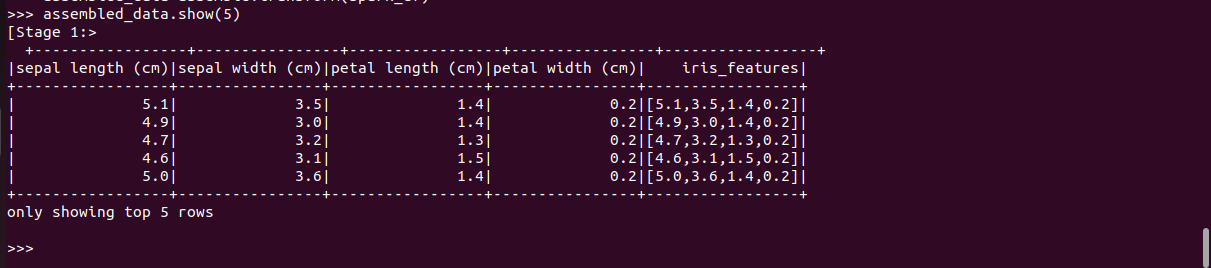
\includegraphics[width=\textwidth]
{NadzuraKumaira/tabel2}
\caption{hasil dari tabel2}
\label{gam:perkuliahan-15-12}
\end{figure}

\begin{figure}
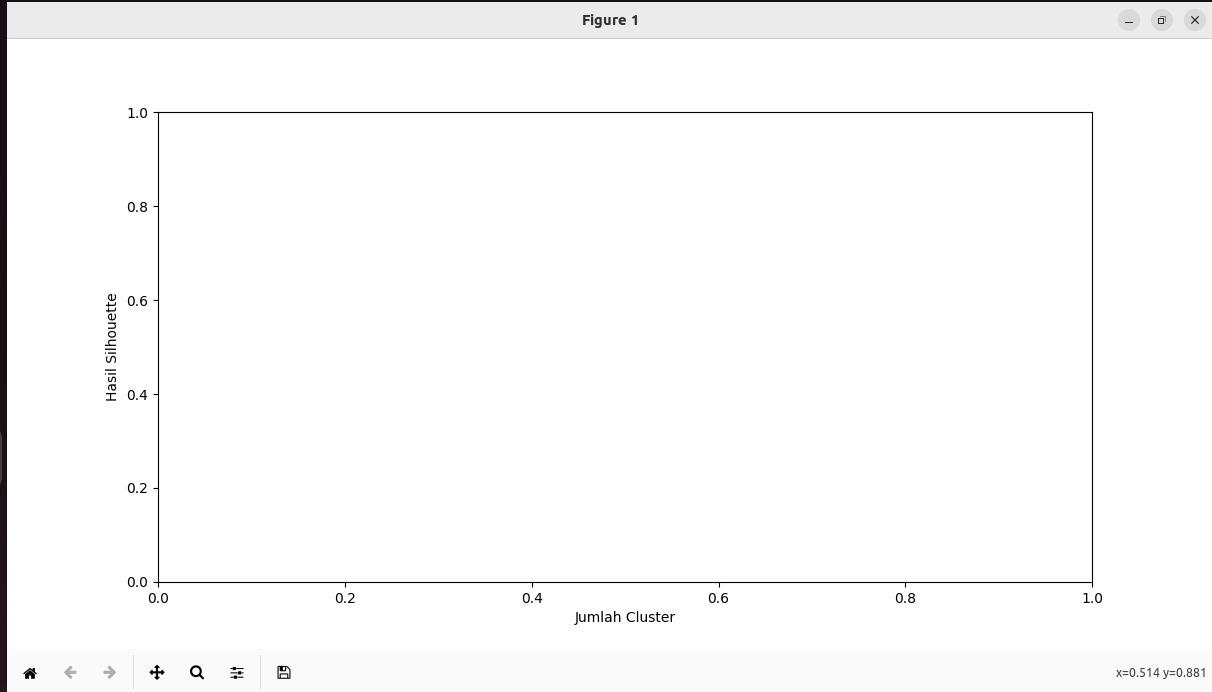
\includegraphics[width=\textwidth]
{NadzuraKumaira/grapik1}
\caption{hasil dari grapik1}
\label{gam:perkuliahan-15-12}
\end{figure}

\begin{figure}
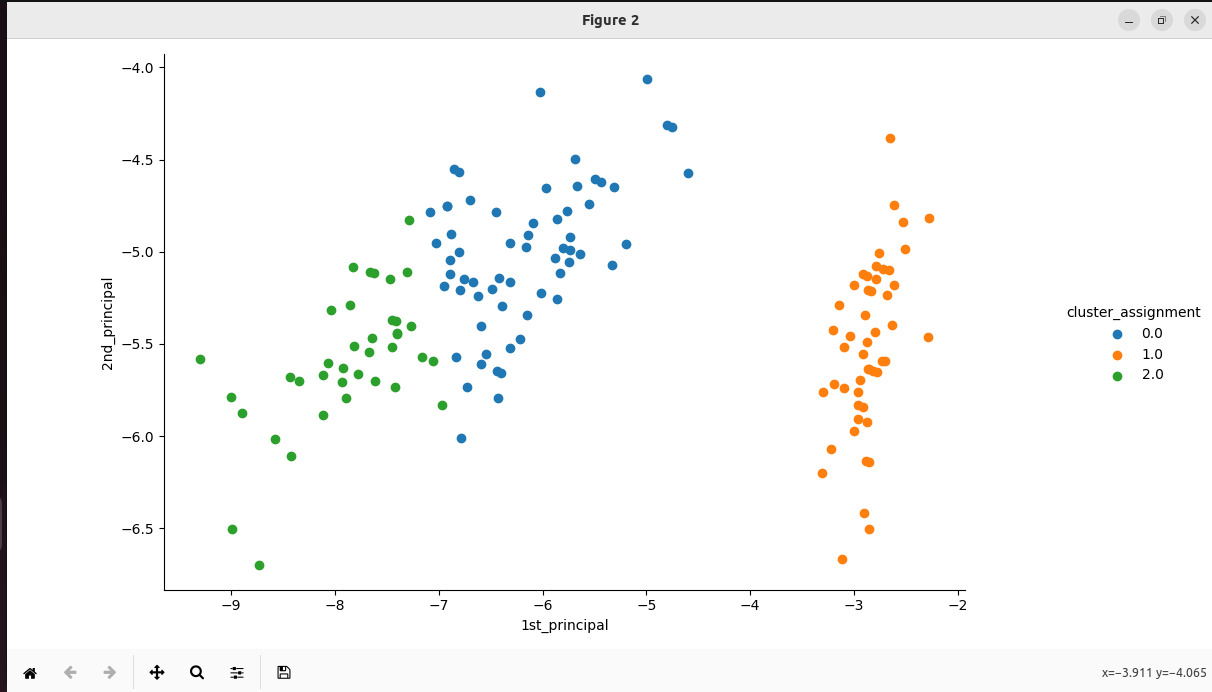
\includegraphics[width=\textwidth]
{NadzuraKumaira/grapik2}
\caption{hasil dari grapik2}
\label{gam:perkuliahan-15-12}
\end{figure}
\end{enumerate}
